%!TEX root = ../modularized/KokkosTutorial_08_KokkosKernels.tex
% \begin{frame}{DOE ECP Acknowledgement}

% \textit{
% This research was supported by the Exascale Computing Project (17-SC-20-SC),
% a joint project of the U.S. Department of Energy's Office of Science and National Nuclear Security Administration,
% responsible for delivering a capable exascale ecosystem, including software, applications, and hardware technology,
% to support the nation's exascale computing imperative.
% }

% \end{frame}

%==============================================================================

\begin{frame}[fragile]


  \vspace{10pt}
  {\Huge Building Applications with Kokkos Kernels}

  \vspace{10pt}

  \textbf{Learning objectives:}
  \begin{itemize}
    \item{Using Kokkos Kernels in Your Project}
    \item{Configure, Build, and Install Kokkos Kernels}
    \item{Install with Spack}
  \end{itemize}

%  \vspace{-20pt}
  \pause

  \begin{block}{Ignore This For Tutorial Only}
     The following details on options to integrate Kokkos into your build process are NOT necessary to know if you just want to do the tutorial.
  \end{block}

\end{frame}

\begin{frame}[fragile]{Options for Building Kokkos Kernels}

\begin{itemize}
\item \textbf{Install via CMake:} For large projects with multiple dependencies installing Kokkos via CMake and then building against it is the best option.
\item \textbf{Build inline via CMake:} This is an option suited for applications which have few dependencies (and no one depending on them) and want to build Kokkos inline with their application.
\item \textbf{Using Spack:} For projects which largely rely on components provided by the Spack package manager.
\end{itemize}
\end{frame}

\begin{frame}[fragile]{KokkosKernels CMake Basics}
\begin{itemize}
\item In the spirit of C++ for \emph{code} performance portability, modern CMake aims for \emph{build system} portability
\item Keep builds simple. Language is always C++ (even if CUDA, HIP, Sycl, ...) and all necessary flags are taken care of for you!
\item Single build system call in your project should configure everything
\vskip0.5cm
\begin{shell}
add_library(myLib goTeamVenture.cpp)
target_link_libraries(myLib PUBLIC 
                     Kokkos::kokkoskernels)
\end{shell}
\vskip0.5cm
\item No need to link to Kokkos itself. Kokkos Kernels transitively applies all Kokkos flags.
\end{itemize}
\end{frame}


\begin{frame}[fragile]{KokkosKernels CMake Basics}
\begin{itemize}
\item Developing large software tools with Kokkos requires handling transitive dependencies properly - thankfully this is fairly seamless with CMake
\item Example: abstraction layers that hide Kokkos details
\item App will still generate Kokkos code and needs all Kokkos flags
\end{itemize}
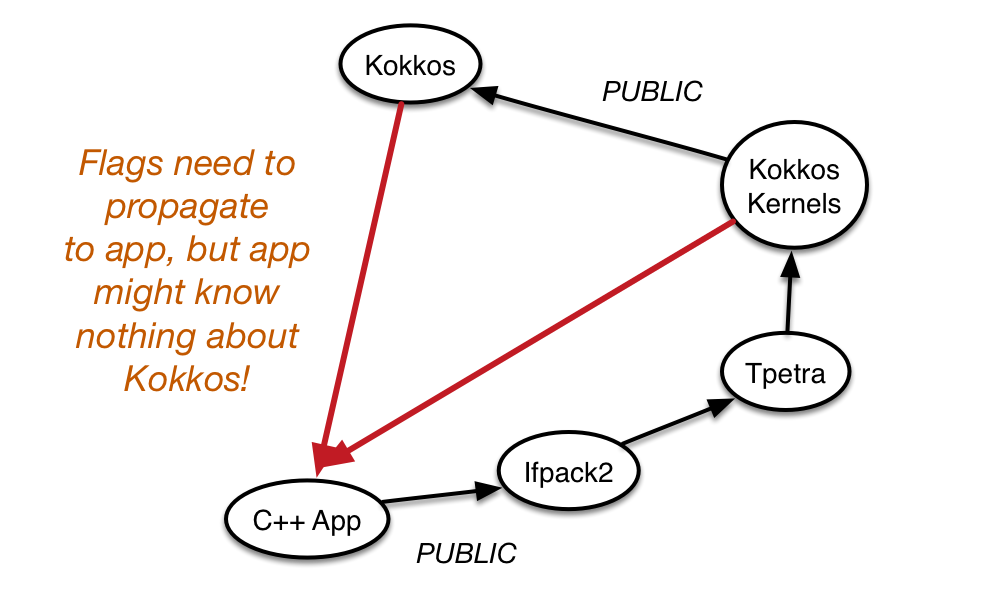
\includegraphics[width=0.6\textwidth]{../figures/DepGraphSimple.png}
\end{frame}

\begin{frame}[fragile]{Project CMake using KokkosKernels}
\textbf{Basic starting point for apps using kernels }
\begin{itemize}
\item Create a \texttt{CMakeLists.txt} file for an executable
\uncover<2-> { \item Declare your C++ project }
\uncover<3-> { \item Find Kokkos Kernels dependency }
\uncover<4-> { \item Add your program }
\uncover<5-> { \item Link to Kokkos Kernels (PRIVATE, not transitive) }
\end{itemize}

\begin{cmake}[linebackground={
  \btLstHL<2>{2}{orange!30}
  \btLstHL<3>{4}{orange!30}
  \btLstHL<4>{6}{orange!30}
  \btLstHL<5>{8-9}{orange!30}    
}]
    cmake_minimum_required(VERSION 3.12)
    project(myProject CXX) # C++ needed to build my project

    find_package(KokkosKernels REQUIRED)

    add_executable(myExe source.cpp)
    # declare dependency on KokkosKernels
    target_link_libraries(myExe PRIVATE 
                 Kokkos::kokkoskernels)
\end{cmake}
\end{frame}

\begin{frame}[fragile]{Project CMake using KokkosKernels}
\textbf{Basic starting point for app using kernels as submodule}
\begin{itemize}
\item Create \texttt{CMakeLists.txt} for a library with Kokkos built inline
\uncover<2-> { \item Declare your C++ project }
\uncover<3-> { \item Add Kokkos as a subdirectory }
\uncover<4-> { \item Add your program  }
\uncover<5-> { \item Link your program to Kokkos Kernels }
\end{itemize}

\begin{cmake}[linebackground={
  \btLstHL<2>{2}{orange!30}
  \btLstHL<3>{4-5}{orange!30}
  \btLstHL<4>{8}{orange!30}
  \btLstHL<5>{10-11}{orange!30}    
}]
    cmake_minimum_required(VERSION 3.12)
    project(myProject CXX) # C++ needed to build my project

    add_subdirectory(kokkos)
    add_subdirectory(kokkos-kernels)

    add_executable(myExe source.cpp)
    # declare dependency on KokkosKernels
    target_link_libraries(myLib PUBLIC 
                 Kokkos::kokkoskernels)
\end{cmake}
\end{frame}

\begin{frame}[fragile]{Project CMake using KokkosKernels}
\textbf{Basic starting point for helper libraries using kernels: PUBLIC dependencies}
\begin{itemize}
\item Create a \texttt{CMakeLists.txt} file for your library
\uncover<2-> { \item Declare your C++ project }
\uncover<3-> { \item Find Kokkos Kernels dependency }
\uncover<4-> { \item Add your library  }
\uncover<5-> { \item Link your library to Kokkos Kernels. Downstream apps will need Kokkos flags so linkage must be PUBLIC (i.e. transitive) }
\end{itemize}

\begin{cmake}[linebackground={
  \btLstHL<2>{2}{orange!30}
  \btLstHL<3>{4}{orange!30}
  \btLstHL<4>{7}{orange!30}
  \btLstHL<5>{9-10}{orange!30}    
}]
    cmake_minimum_required(VERSION 3.12)
    project(myProject CXX)

    find_package(KokkosKernels REQUIRED)

    add_library(myLib source.cpp)
    # declare dependency on KokkosKernels
    target_link_libraries(myLib PUBLIC 
                 Kokkos::kokkoskernels)
\end{cmake}
\end{frame}




\begin{frame}[fragile]{Configuring CMake From Command Line}
\begin{itemize}
\uncover<2-> { \item Point to your project source }
\uncover<3-> { \item Use the same C++ complier as Kokkos }
\uncover<4-> { \item Point to Kokkos Kernels installation  }
\uncover<5-> { \item Pass any Kokkos Kernels options }
\end{itemize}
\begin{shell}[linebackground={
  \btLstHL<2>{1}{orange!30}
  \btLstHL<3>{2}{orange!30}
  \btLstHL<4>{3}{orange!30}
  \btLstHL<5>{4}{orange!30}    
}]
    cmake <ProjectSourceDir> \
      -DCMAKE_CXX_COMPILER=<kokkos dir>/bin/nvcc_wrapper \
      -DKokkosKernels_ROOT=<KokkosInstallPrefix> \
      -DKokkosKernels_<OPTION>:BOOL=ON 
\end{shell}
\end{frame}

\begin{frame}[fragile]{CMake Options Overview}
\begin{itemize}
\item Options almost all fall into one of two categories
\begin{itemize}
	\item ETIs (early template instantiation) options
	\item TPLs (third-party libraries like MKL and cuBLAS)
\end{itemize}
\item Template instantiation pre-generates kernels for certain types to avoid compiler overheads later
\begin{itemize}
	\item Scalars: float, double, complex float, complex double
	\item Ordinals: int, int64\_t
	\item Offsets: int, size\_t
	\item Spaces: CUDA, OpenMP, Serial
	\item Layouts: left, right
\end{itemize}
\item Third-party libraries enable using optimized vendor implementations
\begin{itemize}
	\item MKL
	\item cuBLAS
	\item cuSPARSE
	\item SuperLU
\end{itemize}
\end{itemize}
\end{frame}

\begin{frame}[fragile]{CMake Option Examples}
\begin{itemize}
\item \inlineshell{-DKokkosKernels_INST_MEMSPACE_CUDAUVMSPACE=ON} says to pre-instantiate kernels with CUDA UVM
\item \inlineshell{-DKokkosKernels_INST_FLOAT=ON} says to pre-instantiate kernels with 32-bit floats
\item \inlineshell{-DKokkosKernels_ENABLE_TPL_MKL=ON} for MKL support
\item \inlineshell{-DKokkosKernels_ENABLE_TPL_SUPERLU=ON},  \inlineshell{-DSUPERLU_ROOT=<...>} gives install location for SuperLU
\end{itemize}

\uncover<2->{ \centering Activated options displayed in CMake output }
\begin{uncoverenv}<2->
\begin{shell}
KokkosKernels ETI Types
   Devices:  <OpenMP,HostSpace>
   Scalars:  double
   Ordinals: int
   Offsets:  int;size_t
   Layouts:  LayoutLeft

KokkosKernels TPLs
   BLAS:        /usr/lib/libblas.dylib
   LAPACK:      /usr/lib/liblapack.dylib
\end{shell}
\end{uncoverenv}
\end{frame}




\begin{frame}[fragile]{KokkosKernels via Spack: Command Line}
\begin{itemize}
\item Spack provides a package manager that automatically downloads, configures, and installs package dependencies
\item KokkosKernels itself can be easily installed with specific variants (+) and compilers (\%)
\begin{shell}
spack install kokkos-kernels@develop +openmp %gcc@8.3.0
\end{shell}
\item Good practice is to define ``best variant`` for kokkos in your packages.yaml directory, e.g. for Volta system
\begin{shell}
packages:
   kokkos:
    variants: +cuda +openmp +cuda_lambda +wrapper \
              ^cuda@10.1 cuda_arch=70
    compiler: [gcc@7.2.0]
\end{shell}
\item Build rules in \inlineshell{package.py} automatically map Spack variants to correct CMake options
\item Run \inlineshell{spack info kokkos-kernels} to see full list of variants
\end{itemize}
\end{frame}

\begin{frame}[fragile]{KokkosKernels via Spack: Package Files}
\begin{itemize}
\item Build rules created in a \inlineshell{package.py} file
\item Step 1: Declare dependency on specific version of kokkos (3.x, master, or develop)
\begin{shell}
class myLib(CMakePackage):
  depends_on('kokkos-kernels@3.2')
\end{shell}
\item Step 2: Add build rule pointing to Spack-installed Kokkos and same C++ compiler Kokkos uses
\begin{shell}
def cmake_args(self):
  options = []
  ...
  options.append('-DCMAKE_CXX_COMPILER={}'.format(
     self.spec['kokkos'].kokkos_cxx)
  options.append('-DKokkosKernels_ROOT={}'.format(
     self.spec['kokkos-kernels'].prefix)
  return options
\end{shell}
\item More details can be found in Spack.md in Kokkos repo.
\end{itemize}
\end{frame}

\begin{frame}{Section Summary}

  \begin{itemize}
    \item{Kokkos primary build system is CMake.}
    \item{Kokkos options are transitively passed on, including many necessary compiler options.}
    \item{The Spack package manager does support Kokkos.}
  \end{itemize}

\end{frame}
